%%%%%%%%%%%%%%%%%%%%%%%%%%%%%%%%%%%%%%%%%%%%%%%%%%%%%%%%%%%%%%%%%%%%%%%%%%%%%%%%%%
\begin{frame}[fragile]\frametitle{}
\begin{center}
{\Large Object-Oriented Programming: Concepts}
\end{center}
\end{frame}

%%%%%%%%%%%%%%%%%%%%%%%%%%%%%%%%%%%%%%%%%%%%%%%%%%%%%%%%%%%%%%%%%%%%%%%%%%%%%%%%%%%
\begin{frame}[fragile] \frametitle{Managing Larger Programs}
Procedural programming is:
\begin{itemize}
\item  Sequential code
\item  Conditional code (if statements)
\item  Repetitive code (loops)
\item  Store and reuse (functions)
\end{itemize}
In a very large codebase, object oriented programming is a way to arrange your code so that you
can zoom into 500 lines of the code, and understand it while ignoring the other
999,500 lines of code for the moment.
\end{frame}


%%%%%%%%%%%%%%%%%%%%%%%%%%%%%%%%%%%%%%%%%%%%%%%%%%%%%%%%%%%%%%%%%%%%%%%%%%%%%%%%%%%
\begin{frame}[fragile]\frametitle{Starting with Programs}
\begin{itemize}
\item One way to think about object oriented programming is that we are separating
our program into multiple ``zones''.
\item Each ``zone'' contains some code and data (like a program) and has well defined interactions with the outside world and the other
zones within the program.
\end{itemize}
\end{frame}

%%%%%%%%%%%%%%%%%%%%%%%%%%%%%%%%%%%%%%%%%%%%%%%%%%%%%%%%%%%%%%%%%%%%%%%%%%%%%%%%%%%
\begin{frame}[fragile]\frametitle{Sample program}
\begin{lstlisting}
import urllib.request, urllib.parse, urllib.error
from bs4 import BeautifulSoup
import ssl

# Ignore SSL certificate errors
ctx = ssl.create_default_context()
ctx.check_hostname = False
ctx.verify_mode = ssl.CERT_NONE

url = input('Enter - ')
html = urllib.request.urlopen(url, context=ctx).read()
soup = BeautifulSoup(html, 'html.parser')

# Retrieve all of the anchor tags
tags = soup('a')
for tag in tags:
	print(tag.get('href', None))
\end{lstlisting}
\end{frame}

%%%%%%%%%%%%%%%%%%%%%%%%%%%%%%%%%%%%%%%%%%%%%%%%%%%%%%%%%%%%%%%%%%%%%%%%%%%%%%%%%%%
\begin{frame}[fragile]\frametitle{Subdividing a Problem}
\begin{itemize}
\item One of the advantages of the object oriented approach is that it can hide complexity.
\item For example, while we need to know how to use the urllib and BeautifulSoup code, we do not need to know how those libraries work internally.
\item  It allows us to focus on the part of the problem we need to solve and ignore the other parts of the program.
\end{itemize}




\end{frame}


%%%%%%%%%%%%%%%%%%%%%%%%%%%%%%%%%%%%%%%%%%%%%%%%%%%%%%%%%%%%%%%%%%%%%%%%%%%%%%%%%%%
\begin{frame}[fragile]\frametitle{What's an \emph{object}?}
  \textbf{A Python object is a bundle of variables and functions.}
\begin{itemize}
\item What variable names and functions comprise an object is defined by the object's \emph{class}.

\item From one class specification, many objects can be \emph{instantiated}.  Different instances can assign different values to the object variables.

\item Variables and functions in an instance are collectively called \emph{instance attributes}; functions are also termed \emph{instance methods}.
\end{itemize}

\begin{center}
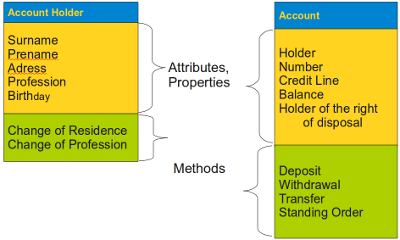
\includegraphics[width=0.5\linewidth,keepaspectratio]{oop1}
\end{center}

% (Ref: https://www.python-course.eu/object\_oriented\_programming.php)
\end{frame}

%%%%%%%%%%%%%%%%%%%%%%%%%%%%%%%%%%%%%%%%%%%%%%%%%%%%%%%%%%%%%%%%%%%%%%%%%%%%%%%%%%%
\begin{frame}[fragile]\frametitle{Encapsulation of Data}

\begin{itemize}
\item Encapsulation is the mechanism for restricting the access to some of an object's components, this means that the internal representation of an object can't be seen from outside of the objects definition. 
\item Access to this data is typically only achieved through methods
\end{itemize}

\begin{center}
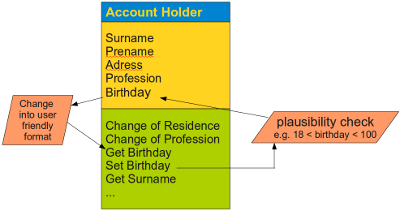
\includegraphics[width=0.5\linewidth,keepaspectratio]{oop2}
\end{center}

% (Ref: https://www.python-course.eu/object\_oriented\_programming.php)
\end{frame}

%%%%%%%%%%%%%%%%%%%%%%%%%%%%%%%%%%%%%%%%%%%%%%%%%%%%%%%%%%%%%%%%%%%%%%%%%%%%%%%%%%%
\begin{frame}[fragile]\frametitle{Inheritance}

\begin{itemize}
\item A class can inherit attributes and behaviour (methods) from other classes, called super-classes.
\item Inheritance: to create new classes by using existing classes. 
\item New ones can both be created by extending and by restricting the existing classes. 
\end{itemize}

\begin{center}
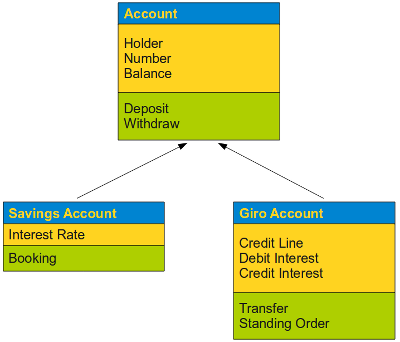
\includegraphics[width=0.5\linewidth,keepaspectratio]{oop3}
\end{center}

% (Ref: https://www.python-course.eu/object\_oriented\_programming.php)
\end{frame}


%%%%%%%%%%%%%%%%%%%%%%%%%%%%%%%%%%%%%%%%%%%%%%%%%%%%%%%%%%%%%%%%%%%%%%%%%%%%%%%%%%%
\begin{frame}[fragile]\frametitle{Using Objects}
Python provides us with many built-in objects.
\begin{lstlisting}
stuff = list()
stuff.append('python')
stuff.append('chuck')
stuff.sort()
print (stuff[0])
print (stuff.__getitem__(0))
print (list.__getitem__(stuff,0))
\end{lstlisting}
The first line is constructing an object of type list, the second and third lines are
calling the \lstinline|append()| method, the fourth line is calling the \lstinline|sort()| method, and the
fifth line is retrieving the item at position 0.
The sixth line is calling the \lstinline|__getitem__()| method in the stuff list with a parameter of zero.
\end{frame}




%%%%%%%%%%%%%%%%%%%%%%%%%%%%%%%%%%%%%%%%%%%%%%%%%%%%%%%%%%%%%%%%%%%%%%%%%%%%%%%%%%%
\begin{frame}[fragile]\frametitle{Example}
Import the \lstinline{date} class from the standard library module \lstinline{datetime}
\begin{lstlisting}
>>> from datetime import date
>>> dt1 = date(2012, 9, 28)
>>> dt2 = date(2012, 10, 1)
\end{lstlisting}
To instantiate an object, call the class name like a function.
\begin{lstlisting}
>>> from datetime import date
>>> dt1 = date(2012, 9, 28)
>>> dt2 = date(2012, 10, 1)
\end{lstlisting}
\end{frame}

%%%%%%%%%%%%%%%%%%%%%%%%%%%%%%%%%%%%%%%%%%%%%%%%%%%%%%%%%%%%%%%%%%%%%%%%%%%%%%%%%%%
\begin{frame}[fragile] \frametitle{Example}
\begin{lstlisting}
>>> dir(dt1)
['__add__', '__class__', 'ctime', 'day',
'fromordinal', 'fromtimestamp', 'isocalendar',
'isoformat', 'isoweekday', 'max', 'min', 'month',
'replace', 'resolution', 'strftime', 'timetuple',
'today', 'toordinal', 'weekday', 'year']
\end{lstlisting}
The \lstinline{dir} function can list all objects attributes. Note there is no distinction between instance variables and methods! Access to object attributes is done by suffixing the instance name with the attribute name, separated by a dot ``\lstinline{.}''.
\begin{lstlisting}
>>> dt1.day
28
>>> dt1.month
9
>>> dt1.year
2012
\end{lstlisting}
\end{frame}

%%%%%%%%%%%%%%%%%%%%%%%%%%%%%%%%%%%%%%%%%%%%%%%%%%%%%%%%%%%%%%%%%%%%%%%%%%%%%%%%%%%
\begin{frame}[fragile]\frametitle{Starting with OOP}
\begin{lstlisting}
class PartyAnimal:
	x = 0
	def party(self) :
		self.x = self.x + 1
		print("So far",self.x)

an = PartyAnimal()
an.party()
an.party()
an.party()
PartyAnimal.party(an)
\end{lstlisting}
When the party method is called, the first parameter (self) points to the particular instance of the PartyAnimal object that party is called from within. 
Within the party method, we see the line:
\lstinline|self.x = self.x + 1|
\end{frame}

%%%%%%%%%%%%%%%%%%%%%%%%%%%%%%%%%%%%%%%%%%%%%%%%%%%%%%%%%%%%%%%%%%%%%%%%%%%%%%%%%%%
\begin{frame}[fragile]\frametitle{Starting with OOP}
Following line is another way to call the party method within
the an object: \lstinline|PartyAnimal.party(an)|
When the program executes, it produces the following output:
\begin{lstlisting}
So far 1
So far 2
So far 3
So far 4
\end{lstlisting}
\end{frame}


%%%%%%%%%%%%%%%%%%%%%%%%%%%%%%%%%%%%%%%%%%%%%%%%%%%%%%%%%%%%%%%%%%%%%%%%%%%%%%%%%%%
\begin{frame}[fragile]\frametitle{The \texttt{self} argument}

  \textbf{Every method of a Python object always has \texttt{self}
    as first argument.}

  
  However, you do not specify it when calling a method: it's
  automatically inserted by Python:
\begin{lstlisting}
>>> class ShowSelf(object):
...   def show(self):
...     print(self)
...
>>> x = ShowSelf() # construct instance
>>> x.show() # `self' automatically inserted!
<__main__.ShowSelf object at 0x299e150>
\end{lstlisting}

  
  The \texttt{self} name is a reference to the object instance
  itself.  You \emph{need to} use \texttt{self} when accessing methods
  or attributes of this instance.
\end{frame}

%%%%%%%%%%%%%%%%%%%%%%%%%%%%%%%%%%%%%%%%%%%%%%%%%%%%%%%%%%%%%%%%%%%%%%%%%%%%%%%%%%%
\begin{frame}[fragile]\frametitle{Member functions}
There are different types of methods/functions.
\begin{lstlisting}
class MyClass:
    def method(self):
        return 'instance method called', self

    @classmethod
    def classmethod(cls):
        return 'class method called', cls

    @staticmethod
    def staticmethod():
        return 'static method called'
\end{lstlisting}
Instead of using a plain class MyClass: declaration you may choose to declare a new-style class inheriting from object with the class MyClass(object):
\end{frame}


%%%%%%%%%%%%%%%%%%%%%%%%%%%%%%%%%%%%%%%%%%%%%%%%%%%%%%%%%%%%%%%%%%%%%%%%%%%%%%%%%%%
\begin{frame}[fragile]\frametitle{Member functions: Instance Methods}

\begin{lstlisting}
class MyClass:
    def method(self):
        return 'instance method called', self
\end{lstlisting}
Through the self parameter, instance methods can freely access attributes and other methods on the same object. 

% (Ref: https://realpython.com/blog/python/instance-class-and-static-methods-demystified/)
\end{frame}


%%%%%%%%%%%%%%%%%%%%%%%%%%%%%%%%%%%%%%%%%%%%%%%%%%%%%%%%%%%%%%%%%%%%%%%%%%%%%%%%%%%
\begin{frame}[fragile]\frametitle{Member functions: Class Methods}
This method is with a @classmethod decorator to flag it as a class method.
\begin{lstlisting}
class MyClass:
    @classmethod
    def classmethod(cls):
        return 'class method called', cls

\end{lstlisting}
  \begin{itemize}
  \item Instead of accepting a self parameter, class methods take a cls parameter that points to the class-and not the object instance-when the method is called.
  \item Because the class method only has access to this cls argument, it can't modify object instance state. 
    \item That would require access to self. However, class methods can still modify class state that applies across all instances of the class.
  \end{itemize}
  
% (Ref: https://realpython.com/blog/python/instance-class-and-static-methods-demystified/)
\end{frame}

%%%%%%%%%%%%%%%%%%%%%%%%%%%%%%%%%%%%%%%%%%%%%%%%%%%%%%%%%%%%%%%%%%%%%%%%%%%%%%%%%%%
\begin{frame}[fragile]\frametitle{Member functions: Static Methods}
Marked with a @staticmethod decorator to flag it as a static method.
\begin{lstlisting}
class MyClass:
    @staticmethod
    def staticmethod():
        return 'static method called'

\end{lstlisting}
  \begin{itemize}
  \item This type of method takes neither a self nor a cls parameter (but of course it's free to accept an arbitrary number of other parameters).
  \item Therefore a static method can neither modify object state nor class state. Static methods are restricted in what data they can access - and they're primarily a way to namespace your methods.
  \end{itemize}
  
% (Ref: https://realpython.com/blog/python/instance-class-and-static-methods-demystified/)
\end{frame}


%%%%%%%%%%%%%%%%%%%%%%%%%%%%%%%%%%%%%%%%%%%%%%%%%%%%%%%%%%%%%%%%%%%%%%%%%%%%%%%%%%%
\begin{frame}[fragile]\frametitle{Member functions: Instance Methods}

\begin{lstlisting}
>>> obj = MyClass()
>>> obj.method()
('instance method called', <MyClass instance at 0x101a2f4c8>)
\end{lstlisting}
This confirmed that method (the instance method) has access to the object instance (printed as ``MyClass instance'') via the self argument.
When the method is called, Python replaces the self argument with the instance object, obj. 

% (Ref: https://realpython.com/blog/python/instance-class-and-static-methods-demystified/)
\end{frame}

%%%%%%%%%%%%%%%%%%%%%%%%%%%%%%%%%%%%%%%%%%%%%%%%%%%%%%%%%%%%%%%%%%%%%%%%%%%%%%%%%%%
\begin{frame}[fragile]\frametitle{Member functions: Instance Methods}

We could ignore the syntactic sugar of the dot-call syntax (obj.method()) and pass the instance object manually to get the same result:

\begin{lstlisting}
>>> MyClass.method(obj)
('instance method called', <MyClass instance at 0x101a2f4c8>)
\end{lstlisting}

% (Ref: https://realpython.com/blog/python/instance-class-and-static-methods-demystified/)
\end{frame}

%%%%%%%%%%%%%%%%%%%%%%%%%%%%%%%%%%%%%%%%%%%%%%%%%%%%%%%%%%%%%%%%%%%%%%%%%%%%%%%%%%%
\begin{frame}[fragile]\frametitle{Member functions: Class Methods}

\begin{lstlisting}
>>> obj.classmethod()
('class method called', <class MyClass at 0x101a2f4c8>)
\end{lstlisting}

  \begin{itemize}
  \item Calling classmethod() showed us it doesn't have access to the ``MyClass instance'' object, but only to the ``class MyClass'' object, representing the class itself (everything in Python is an object, even classes themselves).

  \item Please note that naming these parameters self and cls is just a convention. You could just as easily name them the\_object and the\_class and get the same result. 
  \end{itemize}
  
% (Ref: https://realpython.com/blog/python/instance-class-and-static-methods-demystified/)
\end{frame}

%%%%%%%%%%%%%%%%%%%%%%%%%%%%%%%%%%%%%%%%%%%%%%%%%%%%%%%%%%%%%%%%%%%%%%%%%%%%%%%%%%%
\begin{frame}[fragile]\frametitle{Member functions: Static Methods}

\begin{lstlisting}
>>> obj.staticmethod()
'static method called'
\end{lstlisting}

  \begin{itemize}
  \item Aren't we surprised when they learn that it's possible to call a static method on an object instance.
  \item Behind the scenes Python simply enforces the access restrictions by not passing in the self or the cls argument when a static method gets called using the dot syntax.
  \item This confirms that static methods can neither access the object instance state nor the class state. 
  \item They work like regular functions but belong to the class's (and every instance's) namespace.
  \end{itemize}
% (Ref: https://realpython.com/blog/python/instance-class-and-static-methods-demystified/)
\end{frame}


%%%%%%%%%%%%%%%%%%%%%%%%%%%%%%%%%%%%%%%%%%%%%%%%%%%%%%%%%%%%%%%%%%%%%%%%%%%%%%%%%%%
\begin{frame}[fragile]\frametitle{Member functions: Cases}
When we attempt to call these methods on the class itself - without creating an object instance beforehand:
\begin{lstlisting}
>>> MyClass.classmethod()
('class method called', <class MyClass at 0x101a2f4c8>)

>>> MyClass.staticmethod()
'static method called'

>>> MyClass.method()
TypeError: unbound method method() must
    be called with MyClass instance as first
    argument (got nothing instead)
\end{lstlisting}

  \begin{itemize}
  \item We didn't create an object instance and tried calling an instance function directly on the class blueprint itself. 
  \item This means there is no way for Python to populate the self argument and therefore the call fails.
  \end{itemize}
% (Ref: https://realpython.com/blog/python/instance-class-and-static-methods-demystified/)
\end{frame}

%%%%%%%%%%%%%%%%%%%%%%%%%%%%%%%%%%%%%%%%%%%%%%%%%%%%%%%%%%%%%%%%%%%%%%%%%%%%%%%%%%%
\begin{frame}[fragile]\frametitle{Member functions: Why Static methods?}

\begin{lstlisting}
import math

class Pizza:
    def __init__(self, radius, ingredients):
        self.radius = radius
        self.ingredients = ingredients

    def __repr__(self):
        return (f'Pizza({self.radius!r}, '
                f'{self.ingredients!r})')

    def area(self):
        return self.circle_area(self.radius)

    @staticmethod
    def circle_area(r):
        return r ** 2 * math.pi
\end{lstlisting}

Instead of calculating the area directly within area(), using the well-known circle area formula, I factored that out to a separate circle\_area() static method.

% (Ref: https://realpython.com/blog/python/instance-class-and-static-methods-demystified/)
\end{frame}


%%%%%%%%%%%%%%%%%%%%%%%%%%%%%%%%%%%%%%%%%%%%%%%%%%%%%%%%%%%%%%%%%%%%%%%%%%%%%%%%%%%
\begin{frame}[fragile]\frametitle{Member functions: Why Static methods?}
   \begin{itemize}
  \item As don't take a cls or self argument. That's a big limitation- but it's also a great signal to show that a particular method is independent from everything else around it.
	\item Now, why is that useful?
	\item Flagging a method as a static method is not just a hint that a method won't modify class or instance state - this restriction is also enforced by the Python runtime.
	\item Techniques like that allow you to communicate clearly the intention.
  \end{itemize}

% (Ref: https://realpython.com/blog/python/instance-class-and-static-methods-demystified/)
\end{frame}


%%%%%%%%%%%%%%%%%%%%%%%%%%%%%%%%%%%%%%%%%%%%%%%%%%%%%%%%%%%%%%%%%%%%%%%%%%%%%%%%%%%
\begin{frame}[fragile]\frametitle{Member functions: Properties}
getters and setters:
\begin{lstlisting}
class TestProperty(object):
    def __init__(self, description):
        self._description = description
    @property
    def description(self):
        print 'getting description'
        return self._description
    @description.setter
    def description(self, description):
        print 'setting description'
        self._description = description
\end{lstlisting}
We mark the instance variable as private by prefixing it with an underscore.

The name of the instance variable and the name of the property must be different. If they are not, we get recursion and an error.
\end{frame}

%%%%%%%%%%%%%%%%%%%%%%%%%%%%%%%%%%%%%%%%%%%%%%%%%%%%%%%%%%%%%%%%%%%%%%%%%%%%%%%%%%%
\begin{frame}[fragile]\frametitle{Member function: \_\_init\_\_}
   \begin{itemize}
  \item ``\_\_init\_\_'' is a reseved method in python classes. 
  \item Python doesn't have explicit constructors like C++ or Java, but the \_\_init\_\_() method in Python is something similar, though it is strictly speaking not a constructor. 
  \item It behaves in many ways like a constructor, e.g. it is the first code which is executed, when a new instance of a class is created.
   \end{itemize}
   
\begin{lstlisting}
class Car(object):
	def __init__(self, model, color, company, speed_limit):
		self.color = color
		self.company = company
		self.speed_limit = speed_limit
		self.model = model

\end{lstlisting}

% (Ref: https://micropyramid.com/blog/understand-self-and-\_\_init\_\_-method-in-python-class/)
\end{frame}

%%%%%%%%%%%%%%%%%%%%%%%%%%%%%%%%%%%%%%%%%%%%%%%%%%%%%%%%%%%%%%%%%%%%%%%%%%%%%%%%%%%
\begin{frame}[fragile]\frametitle{Member function: Destructor}
   \begin{itemize}
  \item There is no "real" destructor, but something similiar, i.e. the method \_\_del\_\_. 
  \item It is called when the instance is about to be destroyed. 
  \item If a base class has a \_\_del\_\_() method, the derived class's \_\_del\_\_() method, if any, must explicitly call it to ensure proper deletion of the base class part of the instance. 
   \end{itemize}
   
   
\begin{lstlisting}
class Greeting:
    def __init__(self, name):
        self.name = name
    def __del__(self):
        print "Destructor started"
    def SayHello(self):
        print "Hello", self.name

\end{lstlisting}   
\end{frame}

%%%%%%%%%%%%%%%%%%%%%%%%%%%%%%%%%%%%%%%%%%%%%%%%%%%%%%%%%%%%%%%%%%%%%%%%%%%%%%%%%%%
\begin{frame}[fragile]\frametitle{Member function: Example Construction Destruction}
   
\begin{lstlisting}
>>> from hello_class import Greeting
>>> x1 = Greeting("Guido")
>>> x2 = x1
>>> del x1
>>> del x2
Destructor started   
\end{lstlisting}
   \begin{itemize}
  \item If we use this class, we can see, the "del" doesn't directly call the \_\_del\_\_() method. 
  \item It's apparent that the destructor is not called, when we delete x1. 
  \item The reason is that del decrements the reference count for the object of x1 by one. 
  \item Only if the reference count reaches zero, the destructor is called
     \end{itemize}
\end{frame}



%%%%%%%%%%%%%%%%%%%%%%%%%%%%%%%%%%%%%%%%%%%%%%%%%%%%%%%%%%%%%%%%%%%%%%%%%%%%%%%%%%%
\begin{frame}
  \frametitle{No access control}
  There are no ``public'', ``private'' and 'protected''. qualifiers for object
  attributes.

  
  \textbf{\emph{Any} code can create/read/overwrite/delete \emph{any} attribute on
    \emph{any} object.}

  
  There are \emph{conventions}, though:
  \begin{itemize}
  \item ``protected'' attributes: \texttt{\_name\_}
  \item ``private'' attributes: \texttt{\_\_name\_\_}
  \end{itemize}
  (But again, note that this is not \emph{enforced} by the system in
  any way.)

\end{frame}

%%%%%%%%%%%%%%%%%%%%%%%%%%%%%%%%%%%%%%%%%%%%%%%%%%%%%%%%%%%%%%%%%%%%%%%%%%%%%%%%%%%
 \begin{frame}\frametitle{No overloading}

\begin{itemize}
\item Python does not allow overloading of functions.
\item Any function.
\item Hence, no overloading of constructors.
\item So: \textbf{a class has one and only one constructor.}
\end{itemize}
 \end{frame}


%%%%%%%%%%%%%%%%%%%%%%%%%%%%%%%%%%%%%%%%%%%%%%%%%%%%%%%%%%%%%%%%%%%%%%%%%%%%%%%%%%%
\begin{frame}[fragile]\frametitle{Constructor chaining}
  % \begin{flushright}
  %   \footnotesize%
  %   {\em ``Explicit is better than implicit''}
  %   --- T.~Peters, \href{http://www.python.org/dev/peps/pep-0020/}{The
  %     Zen of Python}
  % \end{flushright}

    When a class is instantiated, Python only calls the first
    constructor it can find in the
    \href{http://www.python.org/download/releases/2.3/mro/}{class inheritance call-chain}.

    %\+ 
    \textbf{If you need to call a parent constructor, you need
      to do it \emph{explicitly}:}
    \begin{lstlisting}
class Application(Task):
  def __init__(self, ...):
    # do Application-specific stuff here
    Task.__init__(self, ...)
    # some more Application-specific stuff
    \end{lstlisting}

    %\+
    Calling a superclass constructor is optional, and
    it can happen anywhere in the init method body.
\end{frame}


%%%%%%%%%%%%%%%%%%%%%%%%%%%%%%%%%%%%%%%%%%%%%%%%%%%%%%%%%%%%%%%%%%%%%%%%%%%%%%%%%%%
\begin{frame}[fragile]\frametitle{Classes as Types}
All variables have a type. And we can use the built-in
dir function to examine the capabilities of a variable. We can use type and dir
with the classes that we create.
\begin{lstlisting}
class PartyAnimal:
	x = 0
	def party(self) :
		self.x = self.x + 1
		print("So far",self.x)

an = PartyAnimal()
print ("Type", type(an))
print ("Dir ", dir(an))
print ("Type", type(an.x))
print ("Type", type(an.party))
\end{lstlisting}
\end{frame}

%%%%%%%%%%%%%%%%%%%%%%%%%%%%%%%%%%%%%%%%%%%%%%%%%%%%%%%%%%%%%%%%%%%%%%%%%%%%%%%%%%%
\begin{frame}[fragile]\frametitle{Object Life-cycle}
As our objects become more complex, we need to take some action within the object to set things up as
the object is being constructed and possibly clean things up as the object is being
discarded.
\begin{lstlisting}
class PartyAnimal:
	x = 0
	def __init__(self):
		print('I am constructed')
	
	def party(self) :
		self.x = self.x + 1
		print('So far',self.x)

	def __del__(self):
		print('I am destructed', self.x)

an = PartyAnimal()
an.party()
an.party()
an = 42
print('an contains',an)
\end{lstlisting}
\end{frame}

%%%%%%%%%%%%%%%%%%%%%%%%%%%%%%%%%%%%%%%%%%%%%%%%%%%%%%%%%%%%%%%%%%%%%%%%%%%%%%%%%%%
\begin{frame}[fragile]\frametitle{Many Instances}
When we are making multiple objects from our class, we might want to set up different initial values for each of the objects.
\begin{lstlisting}
class PartyAnimal:
	x = 0
	name = ''
	def __init__(self, nam):
		self.name = nam
		print(self.name,'constructed')

	def party(self) :
		self.x = self.x + 1
		print(self.name,'party count',self.x)

s = PartyAnimal('Sally')
s.party()
j = PartyAnimal('Jim')
j.party()
s.party()
\end{lstlisting}
\end{frame}

%%%%%%%%%%%%%%%%%%%%%%%%%%%%%%%%%%%%%%%%%%%%%%%%%%%%%%%%%%%%%%%%%%%%%%%%%%%%%%%%%%%
\begin{frame}[fragile]\frametitle{Inheritance}
Ability to create a new class by extending an existing class. When extending a class, we call the
original class the 'parent class' (object) and the new class as the 'child class' (PartyAnimal).
\begin{lstlisting}
class PartyAnimal(object):
	x = 0
	name = ''
	def __init__(self, nam):
		self.name = nam
		print(self.name,'constructed')

	def party(self) :
		self.x = self.x + 1
		print(self.name,'party count',self.x)
\end{lstlisting}
\end{frame}


%%%%%%%%%%%%%%%%%%%%%%%%%%%%%%%%%%%%%%%%%%%%%%%%%%%%%%%%%%%%%%%%%%%%%%%%%%%%%%%%%%%
\begin{frame}[fragile]\frametitle{Child Class}
We can `import' the PartyAnimal class in a new file and extend it as follows:
\begin{lstlisting}
from party import PartyAnimal

class CricketFan(PartyAnimal):
	points = 0

	def six(self):
		self.points = self.points + 6
		self.party()
		print(self.name,"points",self.points)

s = PartyAnimal("Sally")
s.party()
j = CricketFan("Jim")
j.party()
j.six()
print(dir(j))	
\end{lstlisting}
\end{frame}

%%%%%%%%%%%%%%%%%%%%%%%%%%%%%%%%%%%%%%%%%%%%%%%%%%%%%%%%%%%%%%%%%%%%%%%%%%%%%%%%%%%
\begin{frame}[fragile]\frametitle{Inheritance: Try}

\begin{lstlisting}
class Vehicle:
    def __init__(self, name, color):
        self.__name = name      # __name is private to Vehicle class
        self.__color = color
    def getColor(self):         # getColor() function is accessible to class Car
        return self.__color
    def setColor(self, color):  # setColor is accessible outside the class
        self.__color = color
    def getName(self):          # getName() is accessible outside the class
        return self.__name
 
\end{lstlisting}
\end{frame}

%%%%%%%%%%%%%%%%%%%%%%%%%%%%%%%%%%%%%%%%%%%%%%%%%%%%%%%%%%%%%%%%%%%%%%%%%%%%%%%%%%%
\begin{frame}[fragile]\frametitle{Inheritance: Try}

\begin{lstlisting}
class Car(Vehicle):
    def __init__(self, name, color, model):
        # call parent constructor to set name and color  
        super().__init__(name, color)       
        self.__model = model
    def getDescription(self):
        return self.getName() + self.__model + " in " + self.getColor() + " color"
 
# in method getDescrition we are able to call getName(), getColor() because they are 
# accessible to child class through inheritance
c = Car("Ford Mustang", "red", "GT350")
print(c.getDescription())
print(c.getName()) # car has no method getName() but it is accessible through class Vehicle
\end{lstlisting}
\end{frame}



%%%%%%%%%%%%%%%%%%%%%%%%%%%%%%%%%%%%%%%%%%%%%%%%%%%%%%%%%%%%%%%%%%%%%%%%%%%%%%%%%%%
\begin{frame}[fragile]\frametitle{Multiple Inheritance}

A class can inherit from more than one class. 
\begin{lstlisting}
class MySuperClass1():
 
    def method_super1(self):
        print("method_super1 method called")
 
class MySuperClass2():
 
    def method_super2(self):
        print("method_super2 method called")
 
class ChildClass(MySuperClass1, MySuperClass2):
 
    def child_method(self):
        print("child method")
 
c = ChildClass()
c.method_super1()
c.method_super2()
\end{lstlisting}
\end{frame}

%%%%%%%%%%%%%%%%%%%%%%%%%%%%%%%%%%%%%%%%%%%%%%%%%%%%%%%%%%%%%%%%%%%%%%%%%%%%%%%%%%%
\begin{frame}[fragile]\frametitle{Overriding methods}
To override a method in the base class, sub class needs to define a method of same signature. (i.e same method name and same number of parameters as method in base class).

\begin{lstlisting}
class A():
    def __init__(self):
        self.__x = 1
    def m1(self):
        print("m1 from A")
 
class B(A):
    def __init__(self):
        self.__y = 1
    def m1(self):
        print("m1 from B")
 
c = B()
c.m1() # m1 from B
\end{lstlisting}
Try commenting m1()  method  in B  class and now m1()  method from Base class i.e class A  will run.
\end{frame}


%%%%%%%%%%%%%%%%%%%%%%%%%%%%%%%%%%%%%%%%%%%%%%%%%%%%%%%%%%%%%%%%%%%%%%%%%%%%%%%%%%%
\begin{frame}[fragile]\frametitle{isinstance() function}

Used to determine whether the object is an instance of the class or not.
\begin{lstlisting}
>>> isinstance(1, int)
True
 
>>> isinstance(1.2, int)
False
 
>>> isinstance([1,2,3,4], list)
True
\end{lstlisting}

\end{frame}

%%%%%%%%%%%%%%%%%%%%%%%%%%%%%%%%%%%%%%%%%%%%%%%%%%%%%%%%%%%%%%%%%%%%%%%%%%%%%%%%%%%%
%\begin{frame}[fragile] \frametitle{First class objects}
%\begin{itemize}
%\item  All objects in Python are first class. In short, it means there are no restrictions on the object's use. It's the same as any other object.
%\item  Definition, An object is first class if: 
%	\begin{itemize}
%	\item Can be dynamically created, destroyed, 
%	\item passed to a function, returned as a value
%	\end{itemize}
%\item References -- Objects (or references to them) can be shared.  What does this mean?
%	\begin{itemize}
%	\item The object(s) satisfy the identity test operator \lstinline{is}.
%	\item The built-in function \lstinline{id()} returns the same value.
%	\item \lstinline|del()|  -- The built-in function  \lstinline|del()|  removes a reference, not (necessarily)
%the object itself.
%	\end{itemize}
%\end{itemize}
%\end{frame}

%%%%%%%%%%%%%%%%%%%%%%%%%%%%%%%%%%%%%%%%%%%%%%%%%%%%%%%%%%%%%%%%%%%%%%%%%%%%%%%%%%%
\begin{frame}[fragile] \frametitle{Inspection}
\begin{itemize}
\item  Learn what the type of an object is -- Example:  \lstinline|type(obj)|
\item Learn what attributes an object has and what it's capabilities are -- Example: \lstinline|dir(obj)|
\item Get help on a class or an object -- Example:  \lstinline|help(obj)|
\item In Ipython:\lstinline| In [49]: a.upper?|
\end{itemize}
\end{frame}


%%%%%%%%%%%%%%%%%%%%%%%%%%%%%%%%%%%%%%%%%%%%%%%%%%%%%%%%%%%%%%%%%%%%%%%%%%%%%%%%%%%
\begin{frame}[fragile]\frametitle{Exercise}
\begin{itemize}
\item Define a class which has at least two methods:
\item getString: to get a string from console input
\item printString: to print the string in upper case.
\item Also please include simple test function to test the class methods.
\item Hints: Use \_\_init\_\_ method to construct some parameters
\end{itemize}
\end{frame}

%%%%%%%%%%%%%%%%%%%%%%%%%%%%%%%%%%%%%%%%%%%%%%%%%%%%%%%%%%%%%%%%%%%%%%%%%%%%%%%%%%%
\begin{frame}[fragile]\frametitle{Solution}
\begin{lstlisting}
class InputOutString(object):
    def __init__(self):
        self.s = ""

    def getString(self):
        self.s = input()

    def printString(self):
        print self.s.upper()

strObj = InputOutString()
strObj.getString()
strObj.printString()
\end{lstlisting}
\end{frame}

%%%%%%%%%%%%%%%%%%%%%%%%%%%%%%%%%%%%%%%%%%%%%%%%%%%%%%%%%%%%%%%%%%%%%%%%%%%%%%%%%%
\begin{frame}[fragile]\frametitle{}
\begin{center}
{\Large Object Oriented Programming: Examples}
\end{center}
\end{frame}


%%%%%%%%%%%%%%%%%%%%%%%%%%%%%%%%%%%%%%%%%%%%%%%%%%%%%%%%%%%%%%%%%%%%%%%%%%%%%%%%%%%
\begin{frame}[fragile]\frametitle{Recall: \emph{What is a 2D vector?}}

\begin{itemize}
\item A \emph{2D} vector is an element of the vector space $\mathbb{R}^2$.
\item Every \emph{2D} vector $\mathbf{u}$ is completely described by a
  pair of real coordinates $\langle u_x, u_y \rangle$.
\item Note: It is not a point in space. It gives Direction, like a movement recipe. 
\item When added to a point, results into a transformed point.
\end{itemize}
  
  
  
  Two operations are defined on vectors:

  
  \begin{columns}
    \begin{column}{0.6\linewidth}
      \raggedleft
      \emph{vector addition:} if $\mathbf{w} = \mathbf{u} +
        \mathbf{v}$, then $w_x = u_x + v_x$ and $w_y = u_y + v_y$.
    \end{column}
    \begin{column}{0.4\linewidth}
      \centering
      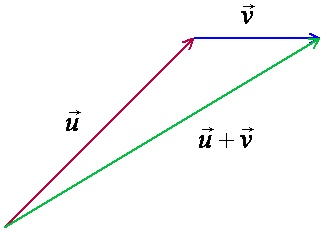
\includegraphics[height=4\baselineskip]{VectorAddition.jpg}
    \end{column}
  \end{columns}

  
  \begin{columns}
    \begin{column}{0.4\linewidth}
      \centering
      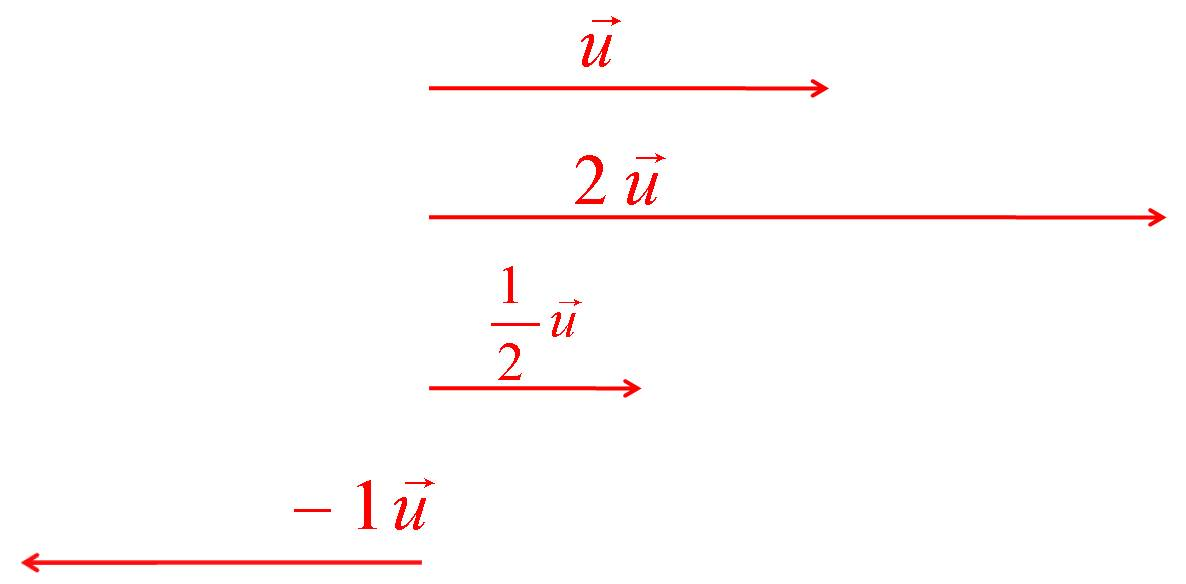
\includegraphics[height=3\baselineskip]{VectorScalarMultiplication.jpg}
    \end{column}
    \begin{column}{0.6\linewidth}
      \raggedright
      \emph{scalar multiplication:} if $\mathbf{v} = \alpha
      \cdot \mathbf{u}$ with $\alpha \in \mathbb{R}$, then $v_x =
      \alpha \cdot u_x$ and $v_y = \alpha \cdot u_y$.
    \end{column}
  \end{columns}

\end{frame}

%%%%%%%%%%%%%%%%%%%%%%%%%%%%%%%%%%%%%%%%%%%%%%%%%%%%%%%%%%%%%%%%%%%%%%%%%%%%%%%%%%%
\begin{frame}[fragile]\frametitle{A \emph{2D vector} in Python}
\begin{lstlisting}
class Vector(object):
 
  def __init__(self, x, y):
    self.x = x
    self.y = y
    
  def add(self, other):
    return Vector(self.x+other.x,
                  self.y+other.y)
                  
  def mul(self, scalar):
    return Vector(scalar*self.x, scalar*self.y)
    
  def show(self):
    return (''<{},{}>''.format(self.x, self.y))
    
\end{lstlisting}
\end{frame}


%%%%%%%%%%%%%%%%%%%%%%%%%%%%%%%%%%%%%%%%%%%%%%%%%%%%%%%%%%%%%%%%%%%%%%%%%%%%%%%%%%%%
%\begin{frame}[fragile]\frametitle{Operations}
%      This identifies user-defined~classes.
%      (Do not leave it out or you'll get an ``old-style'' class, which
%      is deprecated behavior.)
%\begin{lstlisting}
%class Vector(object):
%  """A 2D Vector."""
%  def __init__(self, x, y):
%    self.x = x
%    self.y = y
%  def add(self, other):
%    return Vector(self.x+other.x,
%                  self.y+other.y)
%  def mul(self, scalar):
%    return Vector(scalar*self.x, scalar*self.y)
%  def show(self):
%    return ("<\%g,\%g>" \% (self.x, self.y))
%\end{lstlisting}
%\end{frame}

%%%%%%%%%%%%%%%%%%%%%%%%%%%%%%%%%%%%%%%%%%%%%%%%%%%%%%%%%%%%%%%%%%%%%%%%%%%%%%%%%%%
\begin{frame}[fragile]\frametitle{DocString}
      Classes can have docstrings.
      The content of a class docstring will be shown as help text for
      that class.
\begin{lstlisting}
class Vector(object):
  """A 2D Vector."""
  def __init__(self, x, y):
    self.x = x
    self.y = y
  def add(self, other):
    return Vector(self.x+other.x,
                  self.y+other.y)
  def mul(self, scalar):
    return Vector(scalar*self.x, scalar*self.y)
  def show(self):
    return (''<{},{}>''.format(self.x, self.y))
\end{lstlisting}

\end{frame}


%%%%%%%%%%%%%%%%%%%%%%%%%%%%%%%%%%%%%%%%%%%%%%%%%%%%%%%%%%%%%%%%%%%%%%%%%%%%%%%%%%%
\begin{frame}[fragile]\frametitle{Member functions}
%  \begin{columns}[t]
%    \begin{column}{0.5\linewidth}
\begin{lstlisting}
class Vector(object):
  """A 2D Vector."""
  def __init__(self, x, y):
    self.x = x
    self.y = y
  def add(self, other):
    return Vector(self.x+other.x,
                  self.y+other.y)
  def mul(self, scalar):
    return Vector(scalar*self.x, scalar*self.y)
  def show(self):
    return (''<{},{}>''.format(self.x, self.y))
\end{lstlisting}
%    \end{column}
%    \begin{column}{0.5\linewidth}
%      \raggedleft
      The {\bf def} keyword introduces a method~definition.

      
      Every method \emph{must} have at~least one argument,
      named~{\bf self}.
%    \end{column}
%  \end{columns}
\end{frame}

%%%%%%%%%%%%%%%%%%%%%%%%%%%%%%%%%%%%%%%%%%%%%%%%%%%%%%%%%%%%%%%%%%%%%%%%%%%%%%%%%%%
\begin{frame}[fragile]\frametitle{Exercises}
\begin{itemize}
\item Add a new method \texttt{norm} the \texttt{Vector} class: if
    \texttt{v} is an instance of class \texttt{Vector}, then calling
    \texttt{v.norm()} returns the norm $\sqrt{v_x^2 + v_y^2}$ of
    the associated vector.
\item 
    Add a new method \texttt{unit} to the \texttt{Vector} class: if
    \texttt{v} is an instance of class \texttt{Vector}, then calling
    \texttt{v.unit()} returns the vector \texttt{u} having the
    same direction as \texttt{v} but norm $1$.
\end{itemize}
\end{frame}


%%%%%%%%%%%%%%%%%%%%%%%%%%%%%%%%%%%%%%%%%%%%%%%%%%%%%%%%%%%%%%%%%%%%%%%%%%%%%%%%%%%%
%\begin{frame}[fragile]\frametitle{Recall: 2D Vector}
%  \begin{columns}
%    \begin{column}[t]{0.5\linewidth}
%  We can create vectors by initializing them with the two coordinates
%  $(x,y)$:
%\begin{lstlisting}
%>>> u = Vector(1,0)
%>>> v = Vector(0,1)
%\end{lstlisting}
%    \end{column}
%    \begin{column}[t]{0.5\linewidth}
%      The \lstinline{show} method shows vector coordinates:
%\begin{lstlisting}
%>>> u.show()
%'<1,0>'
%>>> v.show()
%'<0,1>'
%\end{lstlisting}
%    \end{column}
%  \end{columns}
%
%  
%  \begin{columns}
%    \begin{column}[t]{0.5\linewidth}
%      The \lstinline{add} method implements vector addition:
%\begin{lstlisting}
%>>> w = u.add(v)
%>>> w.show()
%'<1,1>'
%\end{lstlisting}
%    \end{column}
%    \begin{column}[t]{0.5\linewidth}
%      The \lstinline{mul} method implements scalar multiplication:
%\begin{lstlisting}
%>>> v2 = v.mul(2)
%>>> v2.show()
%'<0,2>'
%\end{lstlisting}
%    \end{column}
%  \end{columns}
%\end{frame}

%%%%%%%%%%%%%%%%%%%%%%%%%%%%%%%%%%%%%%%%%%%%%%%%%%%%%%%%%%%%%%%%%%%%%%%%%%%%%%%%%%%%
%\begin{frame}[fragile]\frametitle{Name resolution rules, I}
%  \small
%
%  Within a function body, names are resolved according to \href{http://stackoverflow.com/questions/291978/short-description-of-python-scoping-rules/292502#292502}{the LEGB rule}:
%  \begin{description}
%  \item[L] Local scope: any names defined in the current function;
%  \item[E] Enclosing function scope: names defined in enclosing
%    functions (outermost last);
%  \item[G] global scope: names defined in the toplevel of the enclosing module;
%  \item[B] Built-in names (i.e., Python's \texttt{\_\_builtins\_\_} module).
%  \end{description}
%
%  
%  \textbf{Any name that is not in one of the above scopes \emph{must}
%    be qualified.}
%
%  
%  So you have to write \texttt{self.x} to reference an attribute in
%  this instance, \texttt{datetime.date} to mean a class defined in module
%  \texttt{date}, etc.
%
%  % \begin{references}
%  %   \url{http://stackoverflow.com/questions/291978/short-description-of-python-scoping-rules/292502#292502}
%  % \end{references}
%\end{frame}
%
%%%%%%%%%%%%%%%%%%%%%%%%%%%%%%%%%%%%%%%%%%%%%%%%%%%%%%%%%%%%%%%%%%%%%%%%%%%%%%%%%%%%
%\begin{frame}[fragile]\frametitle{Name resolution rules, II}
%      Unqualified name within a function: resolves to a local variable.
%\begin{lstlisting}
%import datetime as dt
%
%def today():
%  td = dt.date.today()
%  return "today is " + td.isoformat()
%
%def hey(name):
%  print("Hey " + name + "; " + today())
%
%hey("you")
%\end{lstlisting}
%
%\end{frame}
%
%%%%%%%%%%%%%%%%%%%%%%%%%%%%%%%%%%%%%%%%%%%%%%%%%%%%%%%%%%%%%%%%%%%%%%%%%%%%%%%%%%%%
%\begin{frame}[fragile]\frametitle{Name resolution rules, III}
%      Unqualified name: since there is no local variable by that name,
%      it resolves to a module-level binding, i.e., to the
%      \texttt{today} function defined above.
%\begin{lstlisting}
%import datetime as dt
%
%def today():
%  td = dt.date.today()
%  return "today is " + td.isoformat()
%
%def hey(name):
%  print("Hey " + name + "; " + today())
%
%hey("you")
%\end{lstlisting}
%
%\end{frame}
%
%%%%%%%%%%%%%%%%%%%%%%%%%%%%%%%%%%%%%%%%%%%%%%%%%%%%%%%%%%%%%%%%%%%%%%%%%%%%%%%%%%%%
%\begin{frame}[fragile]\frametitle{Name resolution rules, IV}
%      Unqualified name: resolves to the \texttt{dt} name created at global scope by the \texttt{import} statement.
%\begin{lstlisting}
%import datetime as dt
%
%def today():
%  td = dt.date.today()
%  return "today is " + td.isoformat()
%
%def hey(name):
%  print("Hey " + name + "; " + today())
%
%hey("you")
%\end{lstlisting}
%
%\end{frame}
%
%%%%%%%%%%%%%%%%%%%%%%%%%%%%%%%%%%%%%%%%%%%%%%%%%%%%%%%%%%%%%%%%%%%%%%%%%%%%%%%%%%%%
%\begin{frame}[fragile]\frametitle{Name resolution rules, V}
%      Qualified name: instructs Python to search the
%      \texttt{date} attribute within the \texttt{dt} module.
%\begin{lstlisting}
%import datetime as dt
%
%def today():
%  td = dt.date.today()
%  return "today is " + td.isoformat()
%
%def hey(name):
%  print("Hey " + name + "; " + today())
%
%hey("you")
%\end{lstlisting}
%
%\end{frame}
%
%%%%%%%%%%%%%%%%%%%%%%%%%%%%%%%%%%%%%%%%%%%%%%%%%%%%%%%%%%%%%%%%%%%%%%%%%%%%%%%%%%%%
%\begin{frame}[fragile]\frametitle{Name resolution rules, VI}
%      Qualified name: Python searches the \texttt{isoformat} attribute
%      within the \texttt{td} object instance.
%\begin{lstlisting}
%import datetime as dt
%
%def today():
%  td = dt.date.today()
%  return "today is " + td.isoformat()
%
%def hey(name):
%  print("Hey " + name + "; " + today())
%
%hey("you")
%\end{lstlisting}
%\end{frame}
%
%%%%%%%%%%%%%%%%%%%%%%%%%%%%%%%%%%%%%%%%%%%%%%%%%%%%%%%%%%%%%%%%%%%%%%%%%%%%%%%%%%%%
%\begin{frame}[fragile]\frametitle{Name resolution rules, VI}
%      Unqualified name: resolves to a local variable in
%      scope of function init
%\begin{lstlisting}
%class Vector(object):
%  def __init__(self, x, y):
%    self.x = x
%    self.y = y
%  # ...
%\end{lstlisting}
%\end{frame}
%
%%%%%%%%%%%%%%%%%%%%%%%%%%%%%%%%%%%%%%%%%%%%%%%%%%%%%%%%%%%%%%%%%%%%%%%%%%%%%%%%%%%%
%\begin{frame}[fragile]\frametitle{Name resolution rules, VII}
%      Qualified names: resolve to attributes in object self.
%
%       (Actually, self.x = ... \emph{creates} the
%      attribute x on self if it does not exist yet.)
%\begin{lstlisting}
%class Vector(object):
%  def __init__(self, x, y):
%    self.x = x
%    self.y = y
%  # ...
%\end{lstlisting}
%
%\end{frame}
%
%%%%%%%%%%%%%%%%%%%%%%%%%%%%%%%%%%%%%%%%%%%%%%%%%%%%%%%%%%%%%%%%%%%%%%%%%%%%%%%%%%%%%
%%\begin{frame}[fragile]\frametitle{Object initialization}
%%      The init method has a special
%%      meaning: it is called when an instance is created.
%%\begin{lstlisting}
%%class Vector(object):
%%  """A 2D Vector."""
%%  def __init__(self, x, y):
%%    self.x = x
%%    self.y = y
%%  def add(self, other):
%%    return Vector(self.x+other.x, self.y+other.y)
%%  def mul(self, scalar):
%%    return Vector(scalar*self.x, scalar*self.y)
%%  def show(self):
%%    return ("<%g,%g>" % (self.x, self.y))
%%\end{lstlisting}
%%\end{frame}
%%
%%
%%%%%%%%%%%%%%%%%%%%%%%%%%%%%%%%%%%%%%%%%%%%%%%%%%%%%%%%%%%%%%%%%%%%%%%%%%%%%%%%%%%%%
%%\begin{frame}[fragile]\frametitle{Constructors}
%%
%%  The init method is the object constructor.
%%  It should \emph{never} return any value.
%%
%%  
%%  You never call init directly, it is invoked by
%%  Python when a new object is created from the class:
%%\begin{lstlisting}
%%# calls Vector.__init__
%%v = Vector(0,1)
%%\end{lstlisting}
%%
%%  
%%  The arguments to init are the arguments you
%%  should supply when creating a class instance.
%%
%%  
%%  (Again, minus the \texttt{self} part which is automatically
%%  inserted by Python.)
%%\end{frame}
%%

%%%%%%%%%%%%%%%%%%%%%%%%%%%%%%%%%%%%%%%%%%%%%%%%%%%%%%%%%%%%%%%%%%%%%%%%%%%%%%%%%%%%
%\begin{frame}[fragile]
%  \frametitle{What we shall see in this part}
%
%  How to use Object-oriented programming for effective code reuse.
%
%  We shall use mainly
%  \href{http://mathworld.wolfram.com/ComplexNumber.html}{complex
%    numbers} as examples.
%\end{frame}

%%%%%%%%%%%%%%%%%%%%%%%%%%%%%%%%%%%%%%%%%%%%%%%%%%%%%%%%%%%%%%%%%%%%%%%%%%%%%%%%%%%
\begin{frame}[fragile]\frametitle{Recall: \emph{What is a complex number?}}

\adjustbox{valign=t}{
\begin{minipage}{0.45\linewidth}
      A complex number $\mathbf{z}$ has the form $\mathbf{z} = z_1 + z_2i$, where \\
      $z_1$ and $z_2$ are real numbers; \\
      $z_1$ is called the real part \\
      and $z_2$ the imaginary part.
\end{minipage}
}
\hfill
\adjustbox{valign=t}{
\begin{minipage}{0.4\linewidth}
\begin{center}
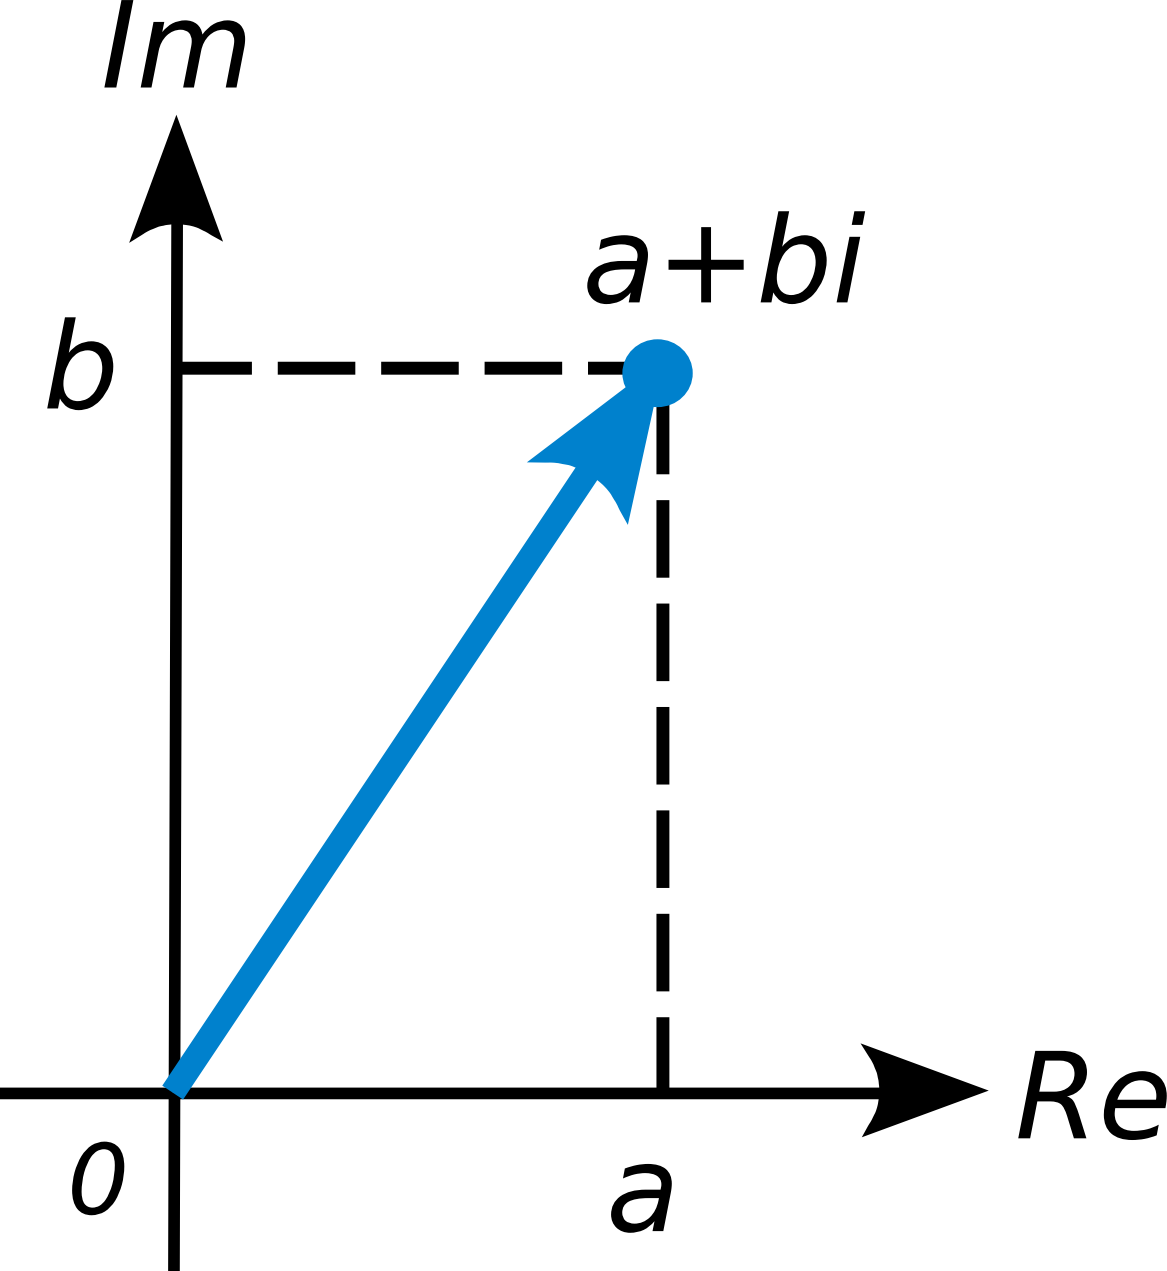
\includegraphics[width=0.8\linewidth,keepaspectratio]{ComplexNumber}
\end{center}
\end{minipage}
}

%
%  \begin{columns}
%    \begin{column}{0.6\linewidth}
%      \raggedleft
%      A complex number $\mathbf{z}$ has the form $\mathbf{z} = z_1 + z_2i$, where \\
%      $z_1$ and $z_2$ are real numbers; \\
%      $z_1$ is called the real part \\
%      and $z_2$ the imaginary part.
%    \end{column}
%    \begin{column}{0.4\linewidth}
%      \centering
%      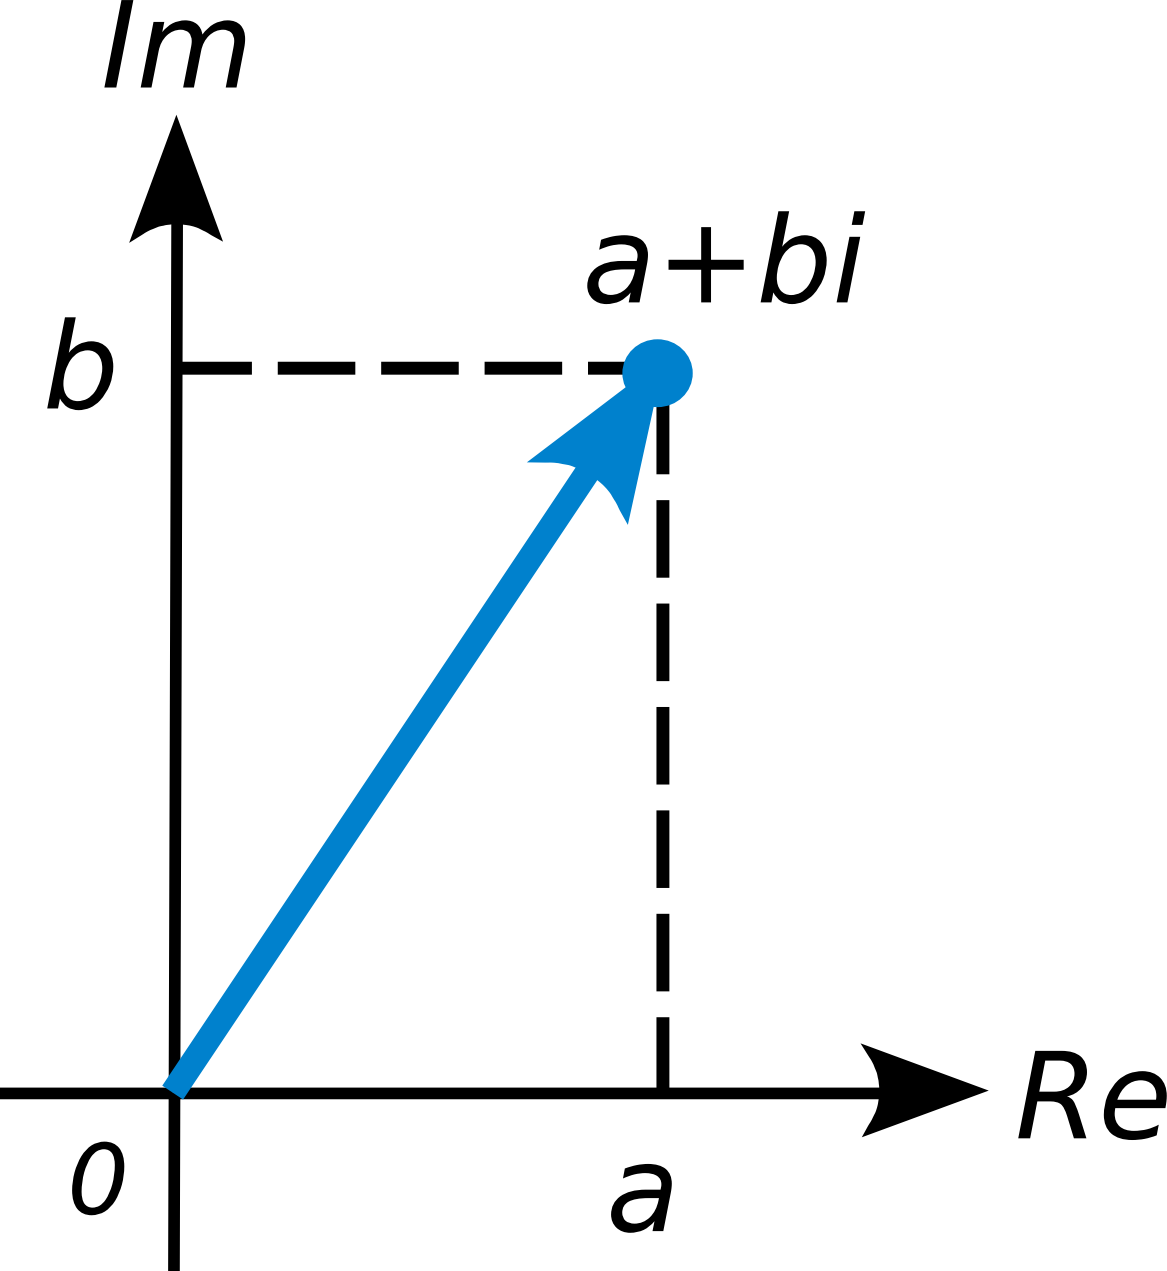
\includegraphics[width=\linewidth]{ComplexNumber}
%    \end{column}
%  \end{columns}

  The set of complex numbers is a field with the two operations:
  \begin{itemize}
  \item
    \emph{addition:} if $\mathbf{z} = \mathbf{x} + \mathbf{y}$, where $\mathbf{x} = x_1 + x_2i$ and $\mathbf{y} = y_1 + y_2i$
    then: $z_1 = x_1 + y_1$, and $z_2 = x_2 + y_2$.

  \item
    \emph{multiplication:} if $\mathbf{z} = \mathbf{x} \cdot
    \mathbf{y}$, then:
 $z_1 = x_1\cdot y_1 - x_2 \cdot y_2$, and $z_2 = x_2\cdot y_1 + x_1\cdot y_2$.
  \end{itemize}
\end{frame}

%%%%%%%%%%%%%%%%%%%%%%%%%%%%%%%%%%%%%%%%%%%%%%%%%%%%%%%%%%%%%%%%%%%%%%%%%%%%%%%%%%%
\begin{frame}[fragile]\frametitle{Naive complex numbers in Python}
 Python object that implements a complex number.
\begin{lstlisting}[showstringspaces=false]
class ComplexNum(object):
  "A complex number z = z1 + z2*i."
  def __init__(self, z1, z2):
    self.re = z1
    self.im = z2
  def __add__(self, other):
    return ComplexNum(
      self.re+other.re, self.im+other.im)
  def __mul__(self, other):
    return ComplexNum(
      self.re*other.re - self.im*other.im,
      self.re*other.im + self.im*other.re)
  def __str__(self):
    return ("%g + %gi" % (self.re, self.im))
  def __eq__(self, other):
    return (self.re == other.re) \
           and (self.im == other.im)
\end{lstlisting}

\end{frame}

%%%%%%%%%%%%%%%%%%%%%%%%%%%%%%%%%%%%%%%%%%%%%%%%%%%%%%%%%%%%%%%%%%%%%%%%%%%%%%%%%%%
\begin{frame}[fragile]\frametitle{What does \texttt{ComplexNum} do?}
  \begin{columns}
    \begin{column}[t]{0.5\linewidth}
      We can create complex numbers by initializing them with the real
      and imaginary part:
\begin{lstlisting}
>>> u = ComplexNum(1,0)
>>> i = ComplexNum(0,1)
>>> z = ComplexNum(1,1)
\end{lstlisting}
    \end{column}
    \begin{column}[t]{0.5\linewidth}
      The str method provides the familiar
      representation:
\begin{lstlisting}
>>> print(u)
1 + 0i
>>> print(i)
0 + 1i
>>> print(z)
1 + 1i
\end{lstlisting}
    \end{column}
  \end{columns}

  %\+
  \begin{columns}
    \begin{column}[t]{0.5\linewidth}
      The add method makes the ``\texttt{+}'' operator work:
\begin{lstlisting}
>>> w = u + i
>>> print(w)
1 + 1i
\end{lstlisting}
    \end{column}
    \begin{column}[t]{0.5\linewidth}
      The mul method makes the ``\texttt{*}'' operator work:
\begin{lstlisting}
>>> m = i*i
>>> print(m)
-1 + 0i
\end{lstlisting}
    \end{column}
  \end{columns}
\end{frame}

%%%%%%%%%%%%%%%%%%%%%%%%%%%%%%%%%%%%%%%%%%%%%%%%%%%%%%%%%%%%%%%%%%%%%%%%%%%%%%%%%%%
\begin{frame}[fragile]\frametitle{Exercises}
\begin{itemize}
\item Add a to\_power method to class \texttt{ComplexNum},
    that takes an integer number as argument and returns the complex
    number raised to that power.

\item 
    Example:
\begin{lstlisting}
>>> z = Complex(1,1)
>>> w = z.to_power(3)
>>> print(w)
-2 + i2
\end{lstlisting}

\item 
Verify that z.to\_power(1),
    z.to\_power(2) and z.to\_power(3) yield the
    same result as z, z*z and
    z*z*z.
\end{itemize}
\end{frame}



%%%%%%%%%%%%%%%%%%%%%%%%%%%%%%%%%%%%%%%%%%%%%%%%%%%%%%%%%%%%%%%%%%%%%%%%%%%%%%%%%%%
\begin{frame}[fragile]\frametitle{Exercises}
%%%%  \begin{exercise}
    Modify the mul method of class \texttt{ComplexNum}:
    \begin{itemize}
    \item If second argument \texttt{other} is an object of class
      \texttt{int} (integer) or \texttt{float} (floating-point
      number) then return the result of scalar multiplication by that number.
    \item If second argument \texttt{other} is an object of class
      \texttt{ComplexNum}, then return the result of complex
      multiplication by that number.
    \end{itemize}
%%%%  \end{exercise}
\end{frame}

%%%%%%%%%%%%%%%%%%%%%%%%%%%%%%%%%%%%%%%%%%%%%%%%%%%%%%%%%%%%%%%%%%%%%%%%%%%%%%%%%%%
\begin{frame}[fragile]\frametitle{\texttt{Vector} vs \texttt{ComplexNum}}

  There's a lot of similarities in the two classes!

  How can we share code between the two?

  \begin{columns}[t]
    \begin{column}{0.5\linewidth}
\begin{lstlisting}[basicstyle=\tiny\ttfamily,showstringspaces=false]
class Vector(object):
  def __init__(self, x, y):
    self.x = x
    self.y = y
  def __eq__(self, other):
    return (self.x == other.x) \
            and (self.y == other.y)
  def __add__(self, other):
    return Vector(
      self.x+other.x, self.y+other.y)
  def __mul__(self, scalar):
    return Vector(
      scalar*self.x,
      scalar*self.y)
  def __str__(self):
    return ("<%g,%g>" % (self.x, self.y))
\end{lstlisting}
    \end{column}
    
    \begin{column}{0.5\linewidth}
\begin{lstlisting}[basicstyle=\tiny\ttfamily,showstringspaces=false]
class ComplexNum(object):
  def __init__(self, z1, z2):
     self.re = z1
     self.im = z2
  def __eq__(self, other):
      return (self.re == other.re) \
           and (self.im == other.im)
  def __add__(self, other):
      return ComplexNum(
      self.re+other.re, self.im+other.im)
  def __mul__(self, other):
    return ComplexNum(
      self.re*other.re - self.im*other.im,
      self.re*other.im + self.im*other.re)
  def __str__(self):
     return ("%g + %gi" % (self.re, self.im))
\end{lstlisting}
    \end{column}
  \end{columns}
\end{frame}


%%%%%%%%%%%%%%%%%%%%%%%%%%%%%%%%%%%%%%%%%%%%%%%%%%%%%%%%%%%%%%%%%%%%%%%%%%%%%%%%%%%
\begin{frame}[fragile]\frametitle{\emph{Vectors} and \emph{Complex Numbers}}

\adjustbox{valign=t}{
\begin{minipage}{0.45\linewidth}
 Complex Numbers are in $1-1$ correspondence with
      points in the real plane $\mathbb{R}^2$: the set $\mathbb{C}$ of
      Complex Numbers is the set of real \emph{2D} vectors.
\end{minipage}
}
\hfill
\adjustbox{valign=t}{
\begin{minipage}{0.4\linewidth}
\begin{center}
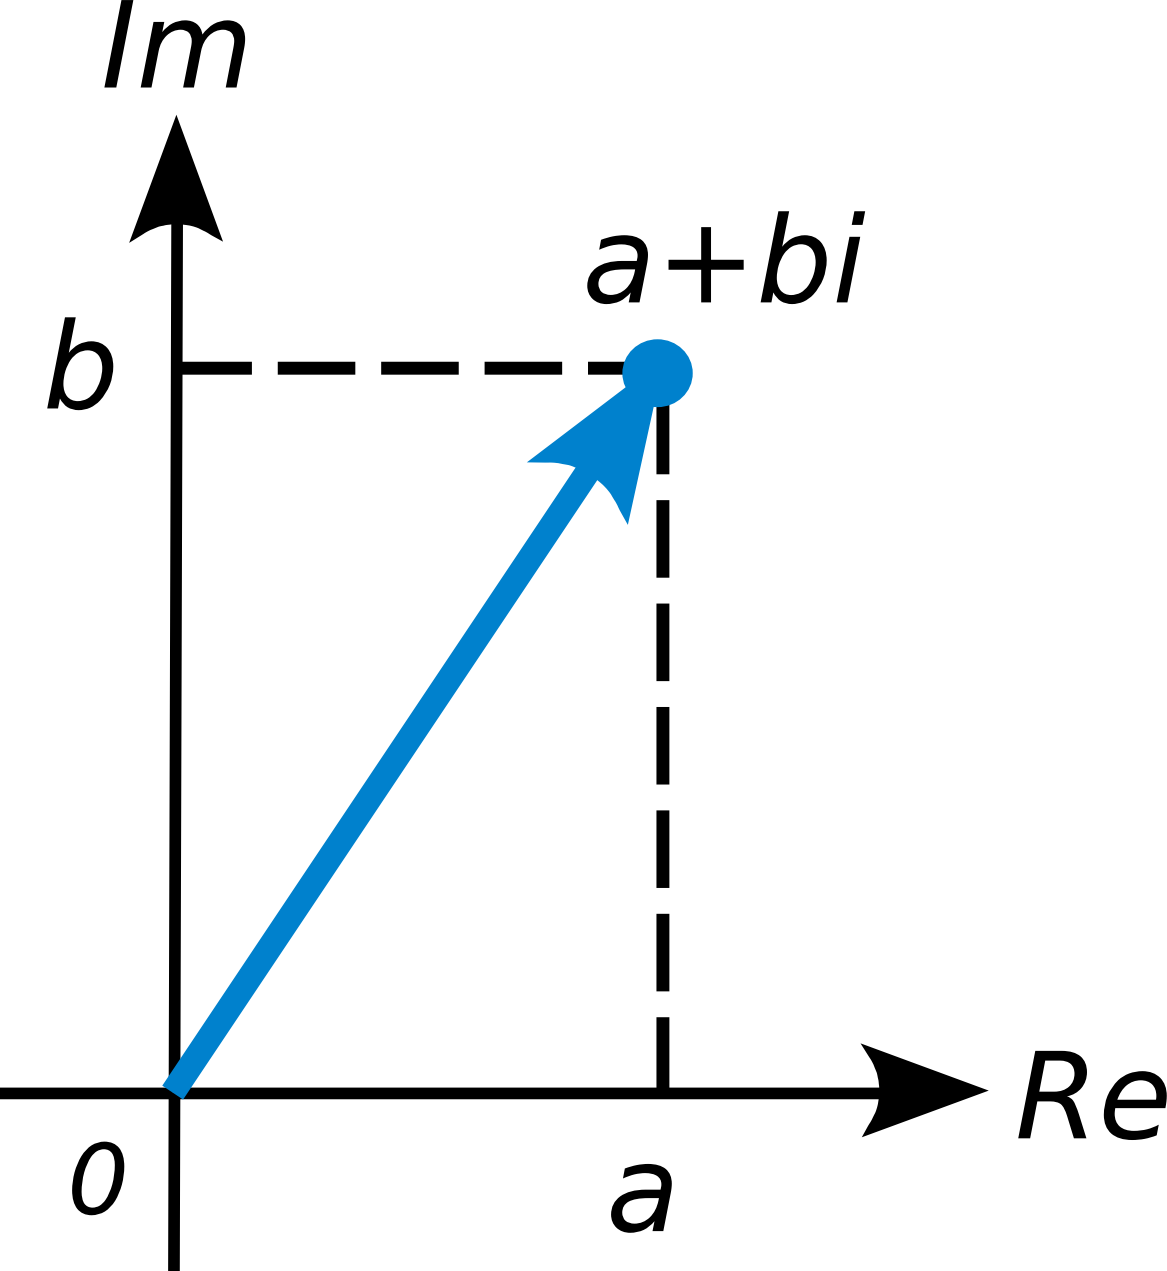
\includegraphics[width=\linewidth,keepaspectratio]{ComplexNumber}
\end{center}
\end{minipage}
}

\begin{itemize}
\item  So we can define the class of Complex Numbers as the class of
  Vectors augmented with a multiplication operation.
\item   So: a Complex Number is a Vector plus some behavior.
\end{itemize}
\end{frame}
%
%%%%%%%%%%%%%%%%%%%%%%%%%%%%%%%%%%%%%%%%%%%%%%%%%%%%%%%%%%%%%%%%%%%%%%%%%%%%%%%%%%%%
%\begin{frame}[fragile]\frametitle{The \texttt{isinstance} function}
%  The \texttt{isinstance($x$, $C$)} function returns \texttt{True} if
%  object $x$ is an instance of class $C$.
%
%  %\+
%  \begin{columns}
%    \begin{column}{0.5\linewidth}
%\begin{lstlisting}
%>>> isinstance(z, ComplexNum)
%True
%>>> isinstance(z, Vector)
%True
%\end{lstlisting}
%    \end{column}
%    \begin{column}{0.4\linewidth}
%      \raggedleft
%      An instance of \texttt{ComplexNum} is also an instance of
%      \texttt{Vector} by inheritance.
%    \end{column}
%  \end{columns}
%\end{frame}
%
%%%%%%%%%%%%%%%%%%%%%%%%%%%%%%%%%%%%%%%%%%%%%%%%%%%%%%%%%%%%%%%%%%%%%%%%%%%%%%%%%%%%
%\begin{frame}[fragile]\frametitle{The \texttt{isinstance} function}
%  The \texttt{isinstance($x$, $C$)} function returns \texttt{True} if
%  object $x$ is an instance of class $C$.
%
%  %\+
%  \begin{columns}
%    \begin{column}{0.5\linewidth}
%\begin{lstlisting}
%>>> isinstance(v, Vector)
%True
%>>> isinstance(v, ComplexNum)
%False
%\end{lstlisting}
%    \end{column}
%    \begin{column}{0.5\linewidth}
%      \raggedleft
%      \emph{However,} instances of \texttt{Vector} are \emph{not}
%      instances of \texttt{ComplexNum}.
%    \end{column}
%  \end{columns}
%\end{frame}
%
%%%%%%%%%%%%%%%%%%%%%%%%%%%%%%%%%%%%%%%%%%%%%%%%%%%%%%%%%%%%%%%%%%%%%%%%%%%%%%%%%%%%
%\begin{frame}[fragile]\frametitle{The \texttt{isinstance} function}
%  The \texttt{isinstance($x$, $C$)} function returns \texttt{True} if
%  object $x$ is an instance of class $C$.
%
%  %\+
%  \begin{columns}
%    \begin{column}{0.5\linewidth}
%\begin{lstlisting}
%>>> isinstance(1, int)
%True
%>>> isinstance(0.5, float)
%True
%>>> isinstance("hi!", str)
%True
%\end{lstlisting}
%    \end{column}
%    \begin{column}{0.5\linewidth}
%      \raggedleft
%      Basic Python objects are instances of built-in classes.
%    \end{column}
%  \end{columns}
%\end{frame}

%%%%%%%%%%%%%%%%%%%%%%%%%%%%%%%%%%%%%%%%%%%%%%%%%%%%%%%%%%%%%%%%%%%%%%%%%%%%%%%%%%%
\begin{frame}[fragile]\frametitle{Inheritance, I}

  \begin{columns}[t]
    \begin{column}{0.5\linewidth}
\begin{lstlisting}[basicstyle=\tiny\ttfamily,showstringspaces=false]
class Vector(object):

  def __init__(self, x, y):
    self.x = x
    self.y = y

  def __eq__(self, other):
    return (self.x == other.x) \
            and (self.y == other.y)

  def __add__(self, other):
    return self.__class__(
      self.x+other.x, self.y+other.y)

  def __mul__(self, scalar):
    return Vector(
      scalar*self.x,
      scalar*self.y)

  def __str__(self):
    return ("<%g,%g>" % (self.x, self.y))
\end{lstlisting}
    \end{column}
    \begin{column}{0.5\linewidth}
\begin{lstlisting}[basicstyle=\tiny\ttfamily,showstringspaces=false]
class ComplexNum(Vector):

  def __mul__(self, other):
    return ComplexNum(
      self.x*other.x - self.y*other.y,
      self.x*other.y + self.y*other.x)

  def __str__(self):
    return ("%g + %gi" % (self.x, self.y))
\end{lstlisting}

\begin{itemize}
\item  \texttt{class ComplexNum} is a
      \emph{child}/\emph{descendant}/\emph{subclass} of class \texttt{Vector}.

\item 
       \texttt{class Vector} is a
      \emph{parent}/\emph{ancestor}/\emph{superclass} of class
      \texttt{ComplexNum}.
\end{itemize}

    \end{column}
  \end{columns}

\end{frame}

%%%%%%%%%%%%%%%%%%%%%%%%%%%%%%%%%%%%%%%%%%%%%%%%%%%%%%%%%%%%%%%%%%%%%%%%%%%%%%%%%%%
\begin{frame}[fragile]\frametitle{Inheritance, II}

  \begin{columns}[t]
    \begin{column}{0.5\linewidth}
\begin{lstlisting}[basicstyle=\tiny\ttfamily,showstringspaces=false]
class Vector(object):

  def __init__(self, x, y):
    self.x = x
    self.y = y

  def __eq__}(self, other):
    return (self.x == other.x) \
            and (self.y == other.y)

  def __add__(self, other):
    return self.__class__(
      self.x+other.x, self.y+other.y)

  def __mul__(self, scalar):
    return Vector(
      scalar*self.x,
      scalar*self.y)

  def __str__(self):
    return ("<%g,%g>" % (self.x, self.y))
\end{lstlisting}
    \end{column}
    \begin{column}{0.5\linewidth}
\begin{lstlisting}[basicstyle=\tiny\ttfamily,showstringspaces=false]
class ComplexNum(Vector):

  def __mul__(self, other):
    return ComplexNum(
      self.x*other.x - self.y*other.y,
      self.x*other.y + self.y*other.x)

  def __str__(self):
    return ("%g + %gi" % (self.x, self.y))
\end{lstlisting}

      %\+
  All methods defined in class \texttt{Vector} are automatically
  defined \emph{(inherited)} in class \texttt{ComplexNum}.
    \end{column}
  \end{columns}
\end{frame}

%%%%%%%%%%%%%%%%%%%%%%%%%%%%%%%%%%%%%%%%%%%%%%%%%%%%%%%%%%%%%%%%%%%%%%%%%%%%%%%%%%%
\begin{frame}[fragile]\frametitle{Inheritance, III}

  \begin{columns}[t]
    \begin{column}{0.5\linewidth}
\begin{lstlisting}[basicstyle=\tiny\ttfamily,showstringspaces=false]
class Vector(object):

  def __init__(self, x, y):
    self.x = x
    self.y = y

  def __eq__(self, other):
    return (self.x == other.x) \
            and (self.y == other.y)

  def __add__(self, other):
    return self.__class__(
      self.x+other.x, self.y+other.y)

  def __mul__(self, other):
    return Vector(
      scalar*self.x,
      scalar*self.y)

  def __str__}(self):
    return ("<%g,%g>" % (self.x, self.y))
\end{lstlisting}
    \end{column}
    \begin{column}{0.5\linewidth}
\begin{lstlisting}[basicstyle=\tiny\ttfamily,showstringspaces=false]
class ComplexNum(Vector):

  def __mul__(self, other):
    return ComplexNum(
      self.x*other.x - self.y*other.y,
      self.x*other.y + self.y*other.x)

  def __str__(self):
    return ("%g + %gi" % (self.x, self.y))
\end{lstlisting}

      \small
      %\+
      Methods mul and str are
      defined in both classes: instances of a class use the
      definition from that class.

      %\+
      We say that \texttt{ComplexNum} \emph{overrides} those
      methods from \texttt{Vector}.
    \end{column}
  \end{columns}
\end{frame}

%%%%%%%%%%%%%%%%%%%%%%%%%%%%%%%%%%%%%%%%%%%%%%%%%%%%%%%%%%%%%%%%%%%%%%%%%%%%%%%%%%%%
%\begin{frame}[fragile]\frametitle{}
%  What happens if a descendant class re-defines a init
%  method?
%
%
%  %\+ 
% {\em
%    The init in the descendant class
%    \emph{overrides} the method in the ancestor class.  So
%    init of the parent class(es) will not be called.
%    }
%\end{frame}



%%%%%%%%%%%%%%%%%%%%%%%%%%%%%%%%%%%%%%%%%%%%%%%%%%%%%%%%%%%%%%%%%%%%%%%%%%%%%%%%%%%
\begin{frame}[fragile]\frametitle{Method chaining}

  Actually, init is not special in this regard.

  %\+ 
  When any instance method is called, Python only calls the first
  constructor it can find in the
  \href{http://www.python.org/download/releases/2.3/mro/}{class
    inheritance call-chain}.

  %\+ 
  \textbf{You can always call a superclass method by prefixing it
    with the superclass name and explicitly writing ``\texttt{self}''
    as the first argument:}
    \begin{lstlisting}
class ComplexNum(Vector):
  # ...
  def print_as_vector(self):
    return Vector.__str__(self)
    \end{lstlisting}
\end{frame}

%%%%%%%%%%%%%%%%%%%%%%%%%%%%%%%%%%%%%%%%%%%%%%%%%%%%%%%%%%%%%%%%%%%%%%%%%%%%%%%%%%%
\begin{frame}[fragile]\frametitle{Inheritance, IV}
Take a look at this Python interaction:
\begin{lstlisting}
>>> z = ComplexNum(1,0)
>>> print(z)
1 + i0
>>> w = ComplexNum(0,1)
>>> print(w)
0 + i1
>>> u = z + w
>>> print(u)
\end{lstlisting}

%\only<1>{\em  What do you think will be printed now?}
%\only<2>{%
%  \vspace{-1.5em}
%\begin{semiverbatim}
%\HL{<1,1>}
%\end{semiverbatim}
 This is no \texttt{ComplexNum}! What's happening here?

\end{frame}

%%%%%%%%%%%%%%%%%%%%%%%%%%%%%%%%%%%%%%%%%%%%%%%%%%%%%%%%%%%%%%%%%%%%%%%%%%%%%%%%%%%
\begin{frame}[fragile]\frametitle{Inheritance, V}
  The answer is in the code:
    \begin{lstlisting}
class Vector(object):
  # ...
  def __add__(self, other):
    return Vector(self.x+other.x, self.y+other.y)
    \end{lstlisting}
    
    The add method returns a new
    Vector instance, even when called from a
    ComplexNum !
\end{frame}

%%%%%%%%%%%%%%%%%%%%%%%%%%%%%%%%%%%%%%%%%%%%%%%%%%%%%%%%%%%%%%%%%%%%%%%%%%%%%%%%%%%
\begin{frame}[fragile]\frametitle{Inheritance, VI}
  Correct code:
    \begin{lstlisting}
class Vector(object):
  # ...
  def __add__(self, other):
    return self.__class__(self.x+other.x, self.y+other.y)
    \end{lstlisting}
    Use the class of the actual instance that's passed,
    instead of hard-coding a class name.
\end{frame}

%%%%%%%%%%%%%%%%%%%%%%%%%%%%%%%%%%%%%%%%%%%%%%%%%%%%%%%%%%%%%%%%%%%%%%%%%%%%%%%%%%%
\begin{frame}[fragile]\frametitle{Polymorphism, I}

  The multiplication operator ``\texttt{*}'' on instances of the
  Vector class works as \emph{scalar multiplication}:
\begin{lstlisting}
>>> v = Vector(1,0)
>>> print (v * 3)
<3,0>
\end{lstlisting}

  %\+
  The same operator ``\texttt{*}'' on instances of the
  ComplexNum class works as \emph{complex multiplication}:
\begin{lstlisting}
>>> z = ComplexNum(1,1)
>>> w = ComplexNum(2,0)
>>> print (z * w)
2 + i2
\end{lstlisting}

  %\+
  \small
  The ability to implement different behavior for the same
  method/operator in different classes is called \emph{polymorphism}.

\end{frame}

%%%%%%%%%%%%%%%%%%%%%%%%%%%%%%%%%%%%%%%%%%%%%%%%%%%%%%%%%%%%%%%%%%%%%%%%%%%%%%%%%%%
\begin{frame}[fragile]\frametitle{Polymorphism, II}

  You may observe that an integer is (in particular) a complex number,
  still we cannot multiply a \texttt{ComplexNum} instance by an
  integer number:
\begin{lstlisting}
>>> print (z * 3)
Traceback (most recent call last):
  File "<stdin>", line 1, in <module>
  File "vector_and_complexnum.py", line 20, in __mul__
    self.x*other.x - self.y*other.y,
AttributeError: 'int' object has no attribute 'x'
\end{lstlisting}

\end{frame}

%%%%%%%%%%%%%%%%%%%%%%%%%%%%%%%%%%%%%%%%%%%%%%%%%%%%%%%%%%%%%%%%%%%%%%%%%%%%%%%%%%%
\begin{frame}[fragile]\frametitle{Polymorphism, III}

\begin{lstlisting}
>>> print (z * 3)
Traceback (most recent call last):
  File "<stdin>", line 1, in <module>
  File "vector_and_complexnum.py", line 20, in __mul__
    self.x*other.x - self.y*other.y,
AttributeError: 'int' object has no attribute 'x'
\end{lstlisting}

  %\+ 
  Our code for mul implicitly assumes
  that argument other has attributes \texttt{x} and
  \texttt{y}, and integers do not!
\end{frame}








%%%%%%%%%%%%%%%%%%%%%%%%%%%%%%%%%%%%%%%%%%%%%%%%%%%%%%%%%%%%%%%%%%%%%%%%%%%%%%%%%%%
\begin{frame}[fragile]\frametitle{Recall: Object Oriented Programming}

\begin{itemize}
\item A Python object is a bundle of variables and functions.
\item Defined  by the object's \emph{class}.
\item  From class, many objects can be \emph{instantiated}.
\item Different instances can assign different values to the object variables.
\end{itemize}
\end{frame}
